\documentclass[cjk,10pt]{beamer}
\usepackage{CJK}
%\usepackage{beamerthemeshadow} %¸ÃΪһÏֳɵÄÄ£°å£¬ÔÚMiKTeX\texmf\tex\latex\beamer\themes\themeÏÂÃæÓкܶà
\usetheme{Warsaw}
\setbeamertemplate{headline}{}{}
\newcommand{\msize}{\scriptsize}
\usepackage{hyperref,amsmath,algorithm,algorithmic,multirow,xcolor}
\usepackage{amsthm,amsmath,enumerate,amsbsy,amsfonts,amssymb,mathabx,amscd,graphicx,algorithm}
\newtheorem{claim}{Claim}
\newtheorem{proposition}{Proposition}
\newtheorem{condition}{Condition}
\begin{document} %ÉêÃ÷ÎĵµµÄ¿ªÊ¼,
\begin{CJK*}{GBK}{song}     %CJK:Ö§³ÖÖÐÎÄ
\title{Web Traffic Time Series Forecasting}
\author{Xin Kang}
\institute{Institute of Statistics and Big Data}
\date{\today}
    \begin{frame} %beamerÀïÖØÒªµÄ¸ÅÄÿ¸öframe¶¨ÒåÒ»ÕÅpage
        \titlepage
    \end{frame}
    \begin{frame}
        \frametitle{Contents}
        \tableofcontents
    \end{frame}
    \section{Introduction}
    \begin{frame}
    \frametitle{Introduction}
    This project focuses on solving the problem of predicting the future web traffic for approximately 145,000 Wikipedia articles. Detailed data description is covered in the following section. Making future prediction on sequential or temporal observations has emerged in many key real-world problems. By forecasting the future values of multiple web traffic time series, we can answer some questions like how many severs you need in reality and what your total cost for next month is when you need to use external severs. If the performance is satisfactory, similar methods can be applied to other websites to predict their web traffic, and it can help people make smart advertisement decisions and make profit.
    \end{frame}
    \section{Exploratory Data Analysis}
    \begin{frame}
    \frametitle{Exploratory Data Analysis}
    \begin{figure}[htbp]
\centering
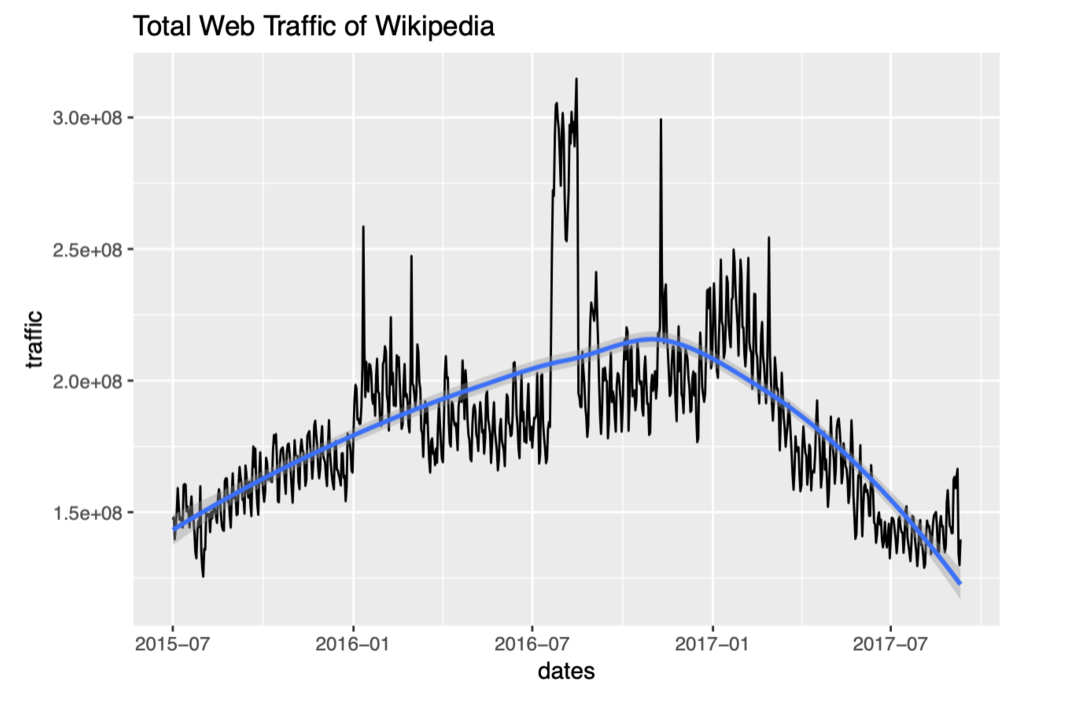
\includegraphics[height=6cm, width=10cm]{1}
\caption{1}
\end{figure}
       \end{frame}
    \begin{frame}
        \frametitle{Exploratory Data Analysis}
    \begin{figure}[htbp]
\centering
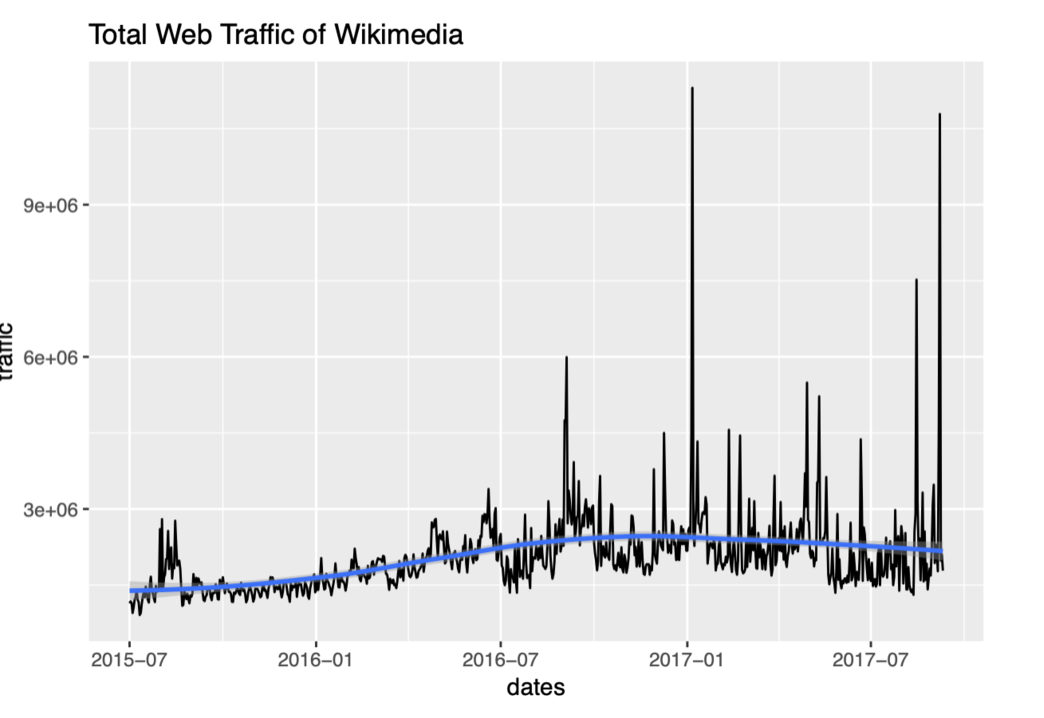
\includegraphics[height=6cm, width=10cm]{2}
\caption{2}
\end{figure}
       \end{frame}
       \begin{frame}
        \frametitle{Exploratory Data Analysis}
    \begin{figure}[htbp]
\centering
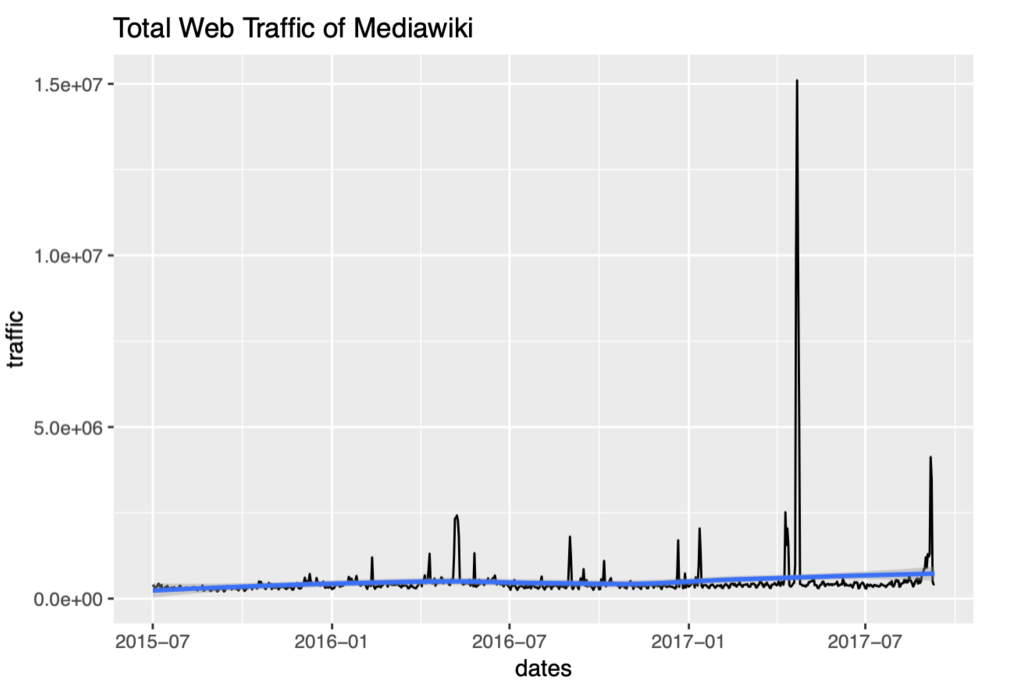
\includegraphics[height=6cm, width=10cm]{3}
\caption{3}
\end{figure}
       \end{frame} 
        \begin{frame}
        \frametitle{Exploratory Data Analysis}
    \begin{figure}[htbp]
\centering
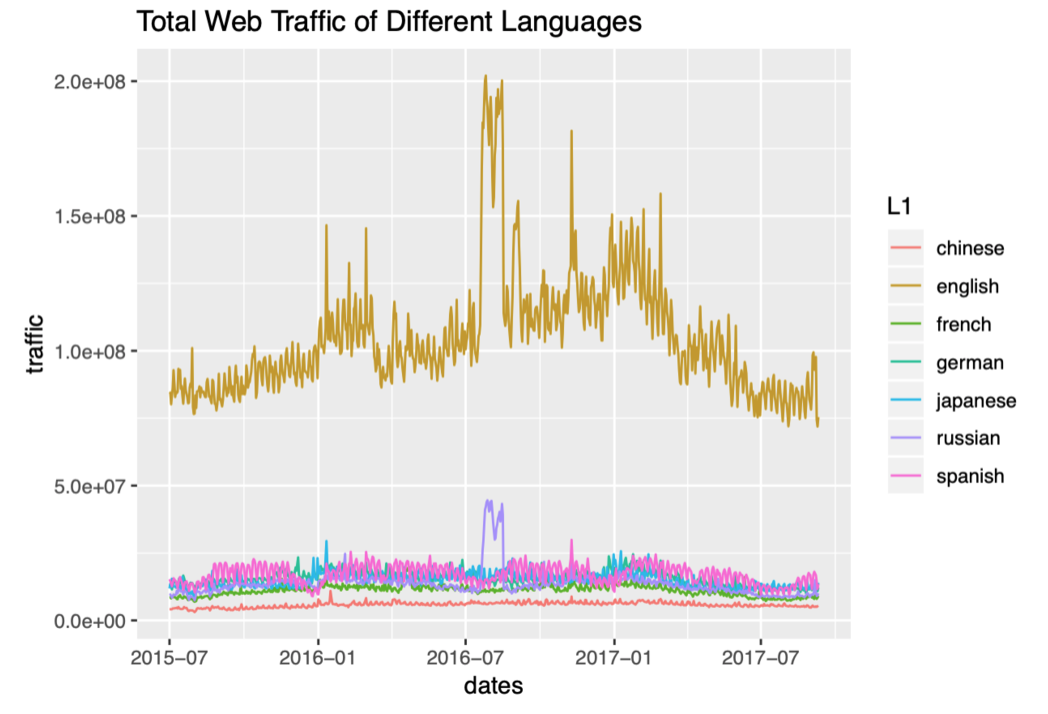
\includegraphics[height=6cm, width=10cm]{4}
\caption{4}
\end{figure}
       \end{frame}
        \begin{frame}
        \frametitle{Exploratory Data Analysis}
    \begin{figure}[htbp]
\centering
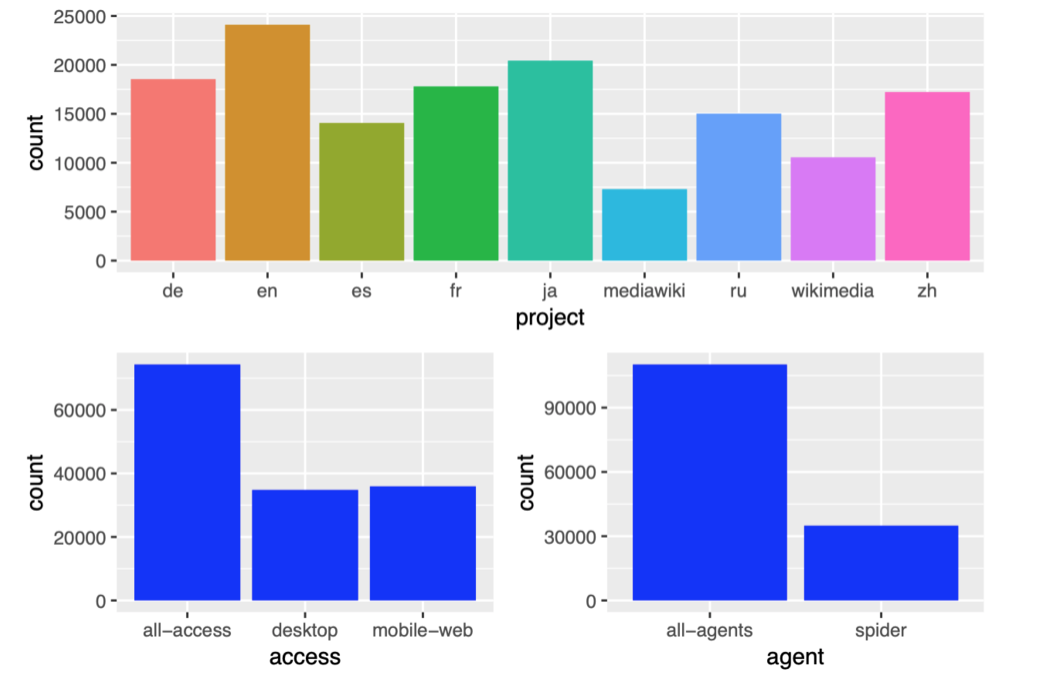
\includegraphics[height=6cm, width=10cm]{5}
\caption{5}
\end{figure}
       \end{frame}
           \begin{frame}
        \frametitle{Exploratory Data Analysis}
    \begin{figure}[htbp]
\centering
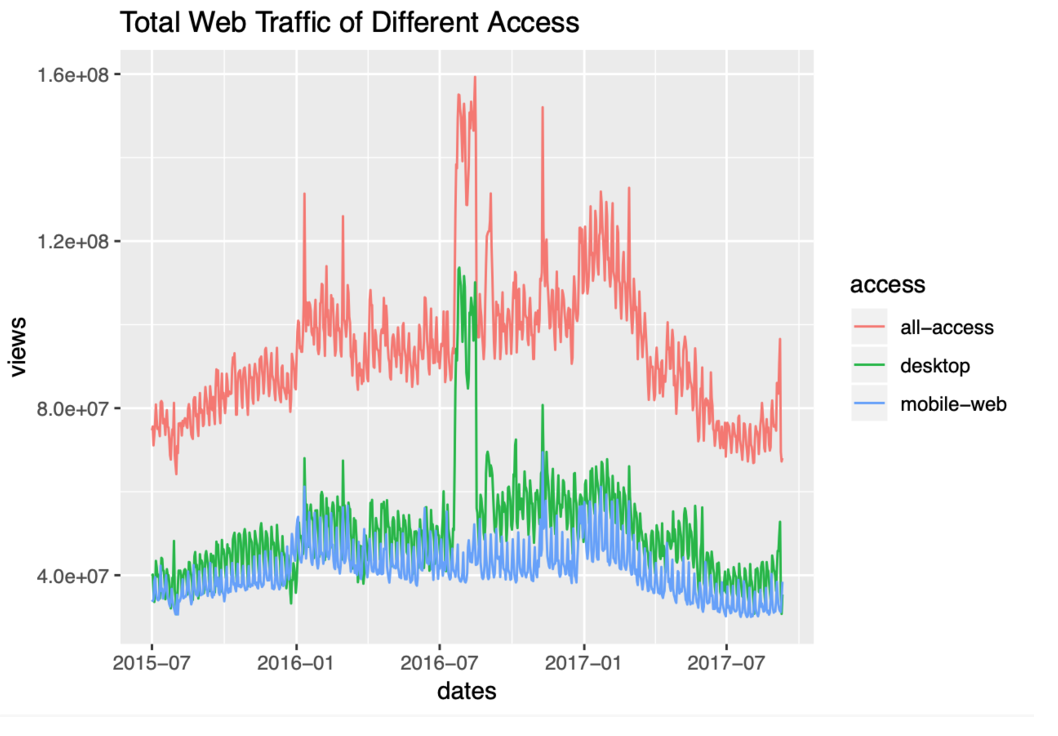
\includegraphics[height=6.5cm, width=10cm]{6}
\caption{6}
\end{figure}
       \end{frame}
            \begin{frame}
        \frametitle{Exploratory Data Analysis}
    \begin{figure}[htbp]
\centering
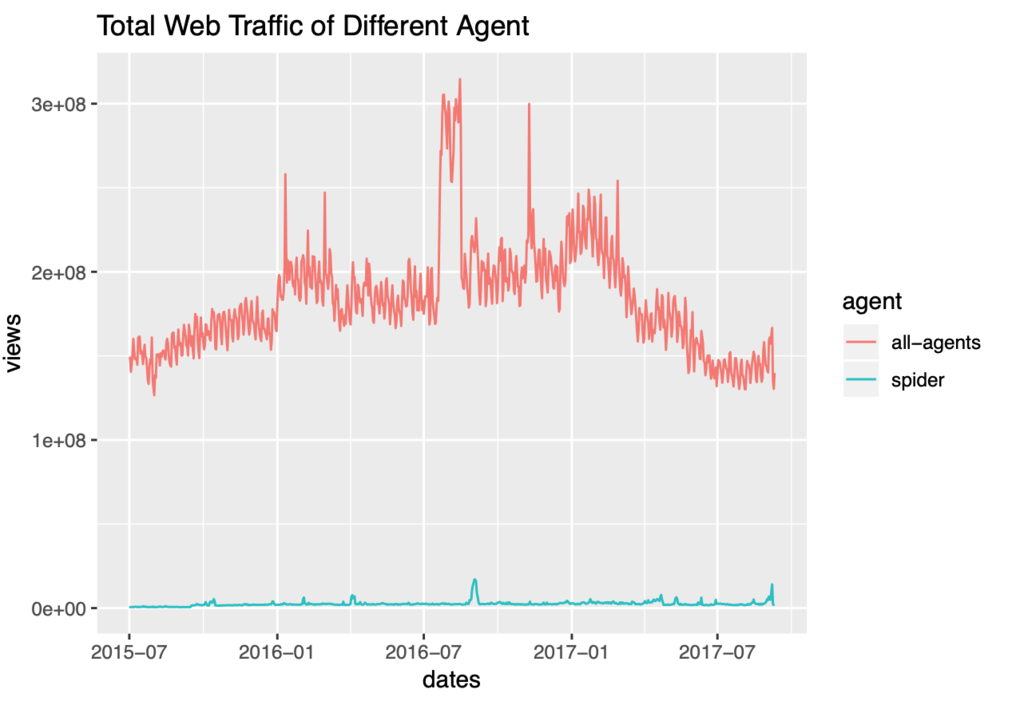
\includegraphics[height=6.5cm, width=10cm]{7}
\caption{7}
\end{figure}
       \end{frame}
             \begin{frame}
        \frametitle{Exploratory Data Analysis}
    \begin{figure}[htbp]
\centering
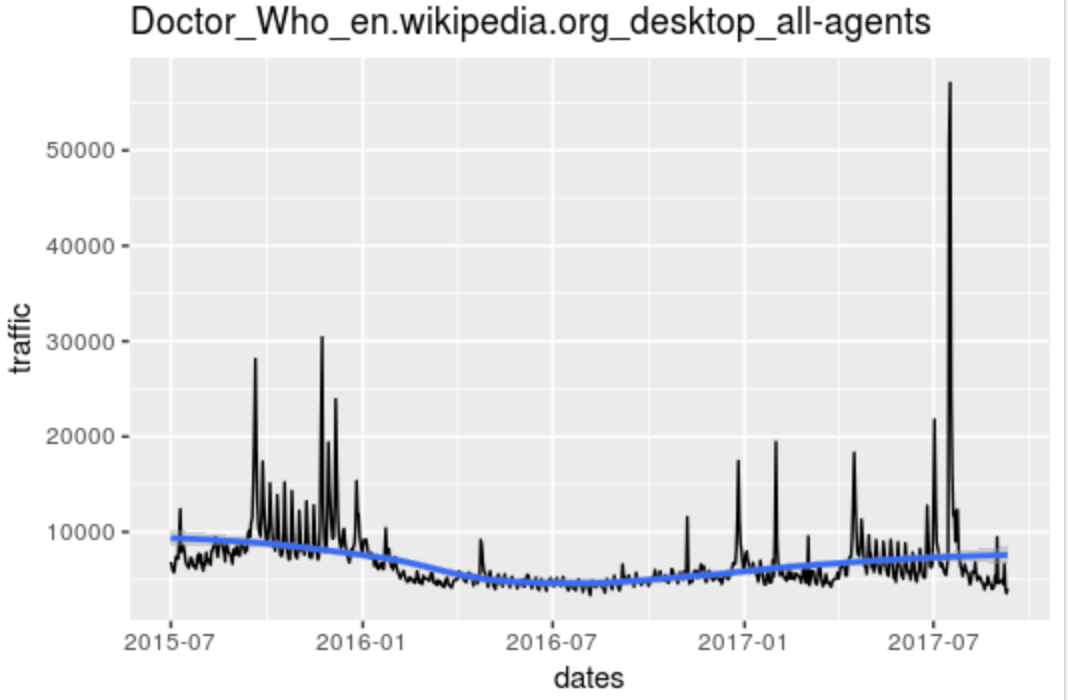
\includegraphics[height=6.5cm, width=10cm]{8}
\caption{8}
\end{figure}
       \end{frame}
              \begin{frame}
        \frametitle{Exploratory Data Analysis}
    \begin{figure}[htbp]
\centering
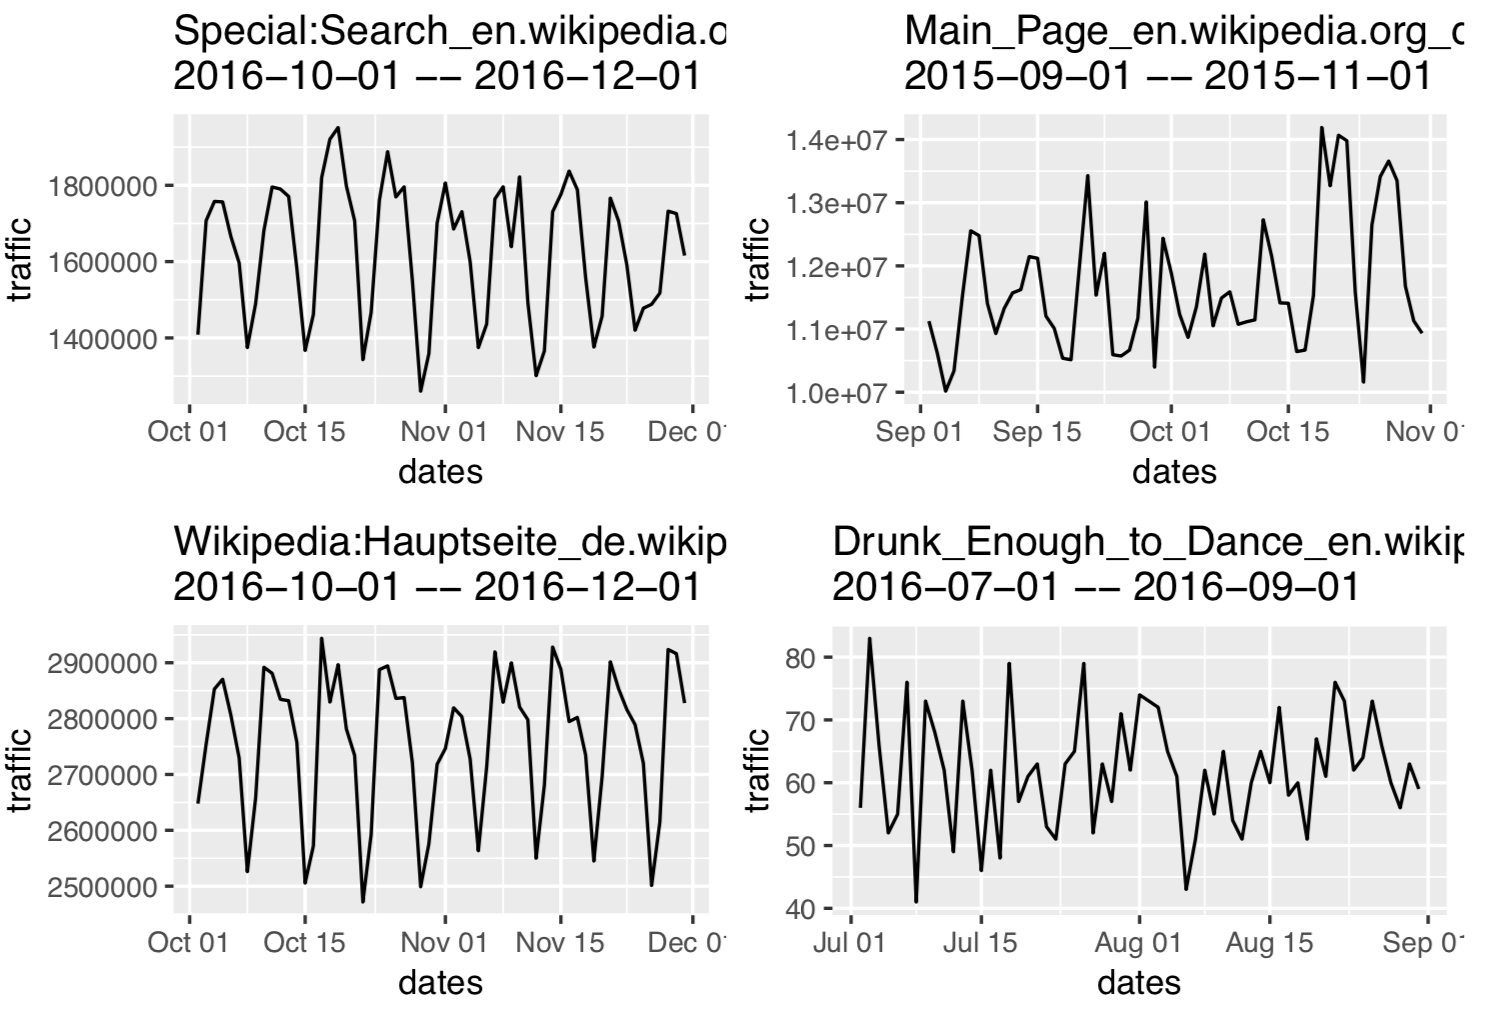
\includegraphics[height=6.5cm, width=10cm]{9}
\caption{9}
\end{figure}
       \end{frame}      
 \section{Model Fitting}
 \subsection{ARIMA}
    \begin{frame}
    \frametitle{Model Fitting -- ARIMA}
    \begin{figure}[htbp]
\centering
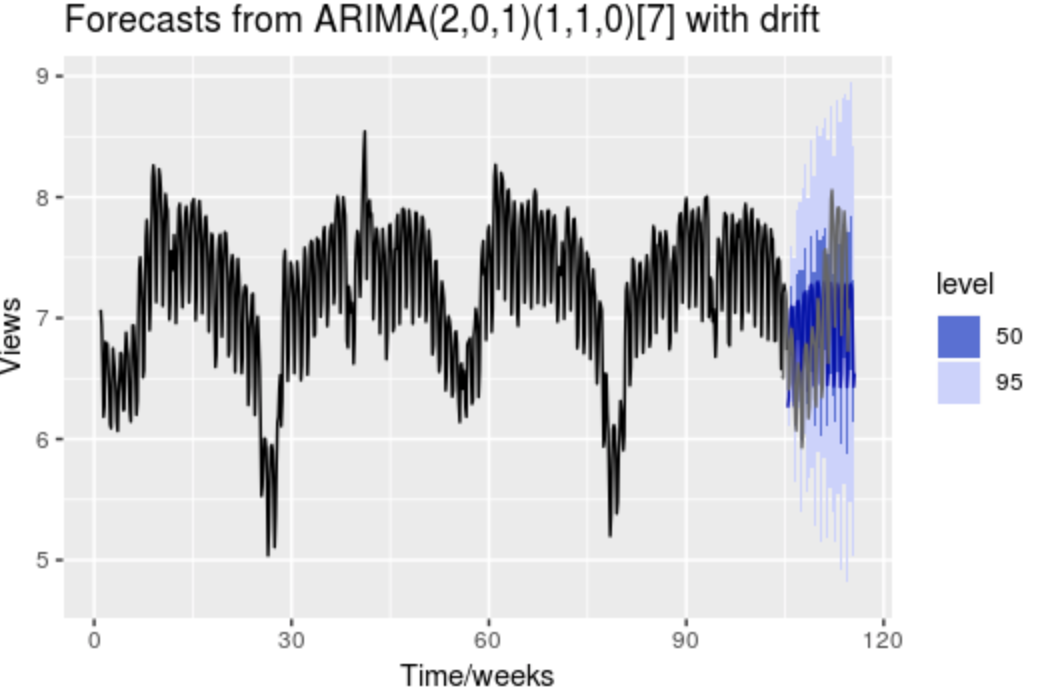
\includegraphics[height=6cm, width=10cm]{10}
\caption{10}
\end{figure}
       \end{frame}
     \begin{frame}
    \frametitle{Model Fitting -- ARIMA}
    \begin{figure}[htbp]
\centering
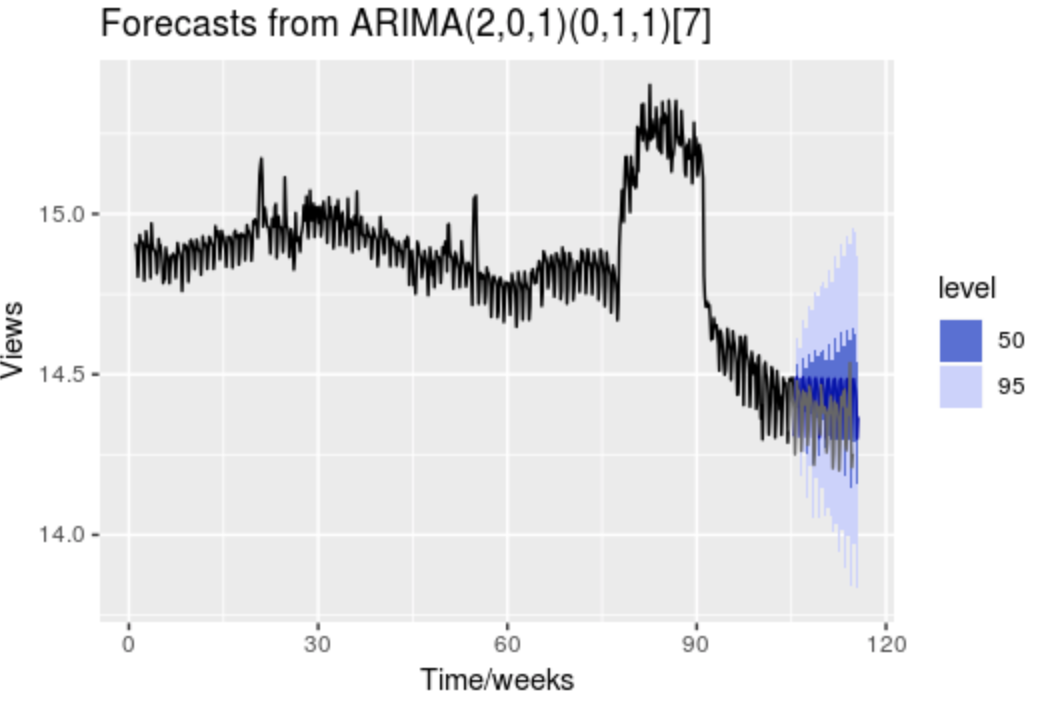
\includegraphics[height=6cm, width=10cm]{11}
\caption{11}
\end{figure}
       \end{frame}  
        \begin{frame}
    \frametitle{Model Fitting -- ARIMA}
    \begin{figure}[htbp]
\centering
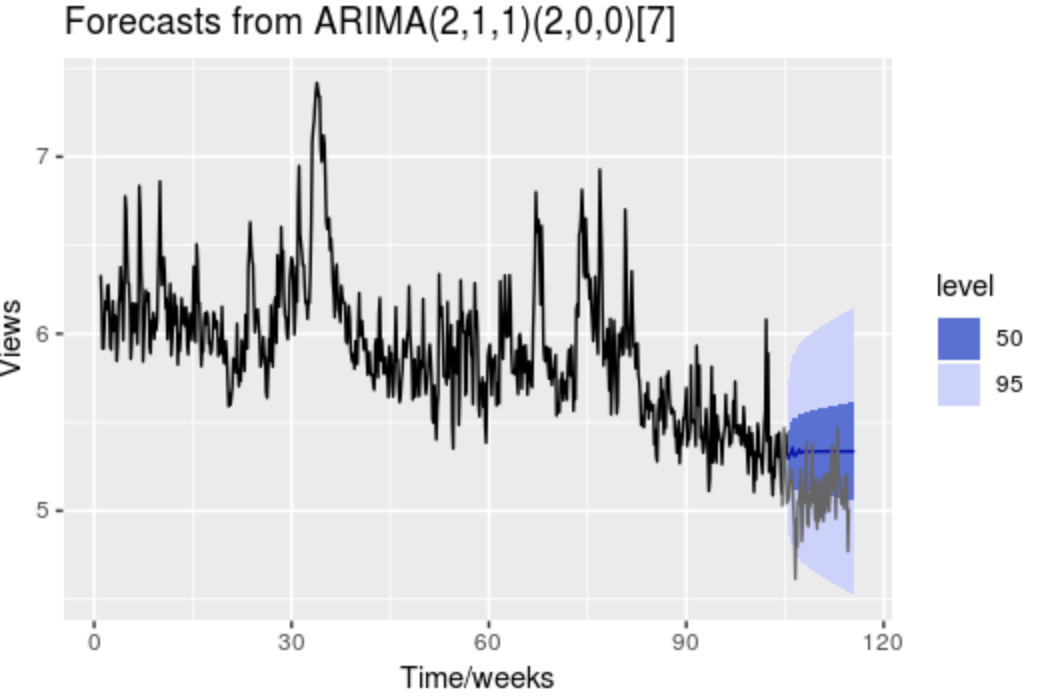
\includegraphics[height=6cm, width=10cm]{12}
\caption{12}
\end{figure}
       \end{frame}
    \begin{frame}
    \frametitle{Model Fitting -- ARIMA}
    \begin{figure}[htbp]
\centering
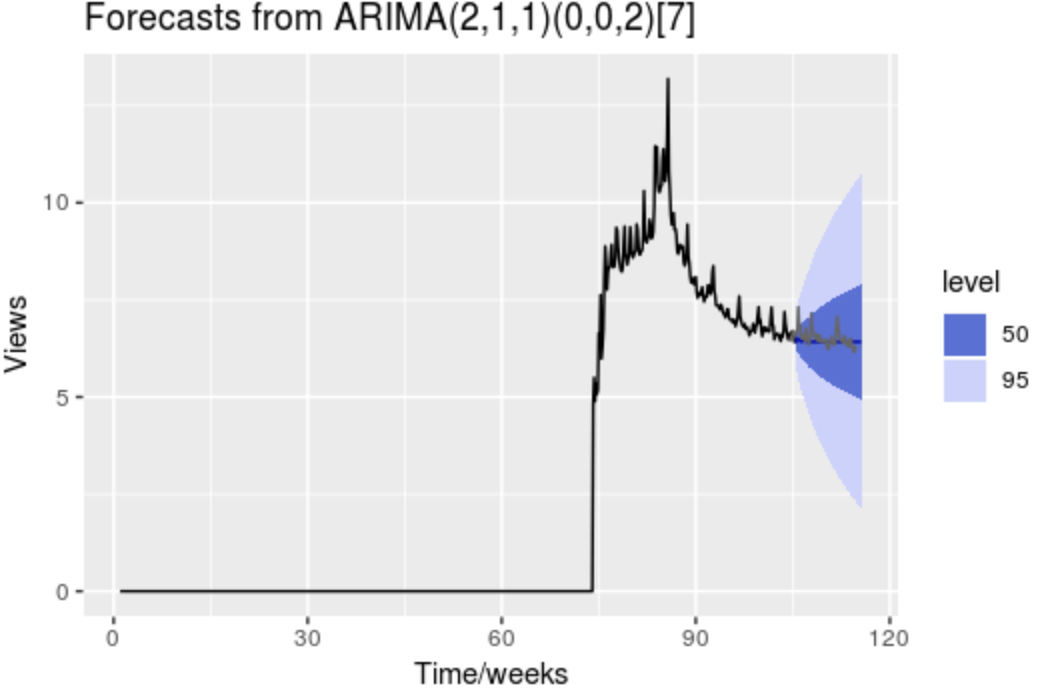
\includegraphics[height=6cm, width=10cm]{13}
\caption{13}
\end{figure}
       \end{frame}    
    \subsection{LSTM}
 \begin{frame}
    \frametitle{Model Fitting -- LSTM}
    \begin{figure}[htbp]
\centering
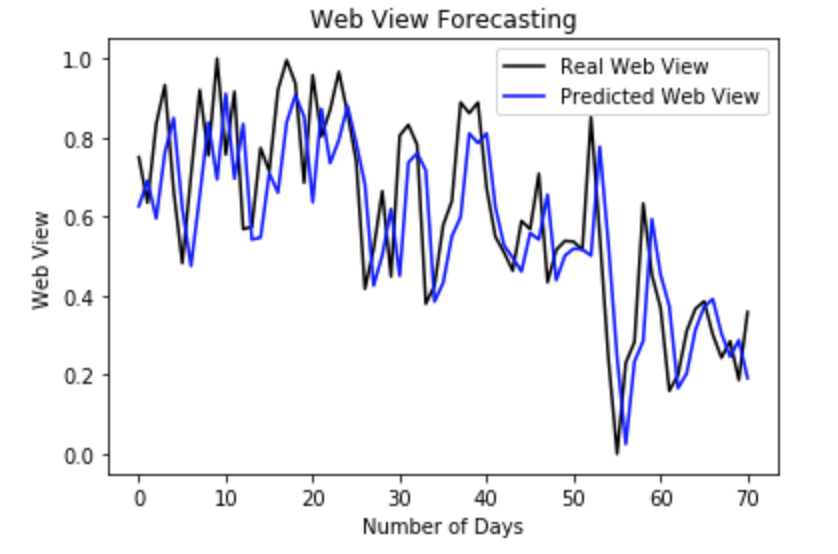
\includegraphics[height=6cm, width=10cm]{14}
\caption{14}
\end{figure}
       \end{frame}    
  \begin{frame}
    \frametitle{Model Fitting -- LSTM}
    \begin{figure}[htbp]
\centering
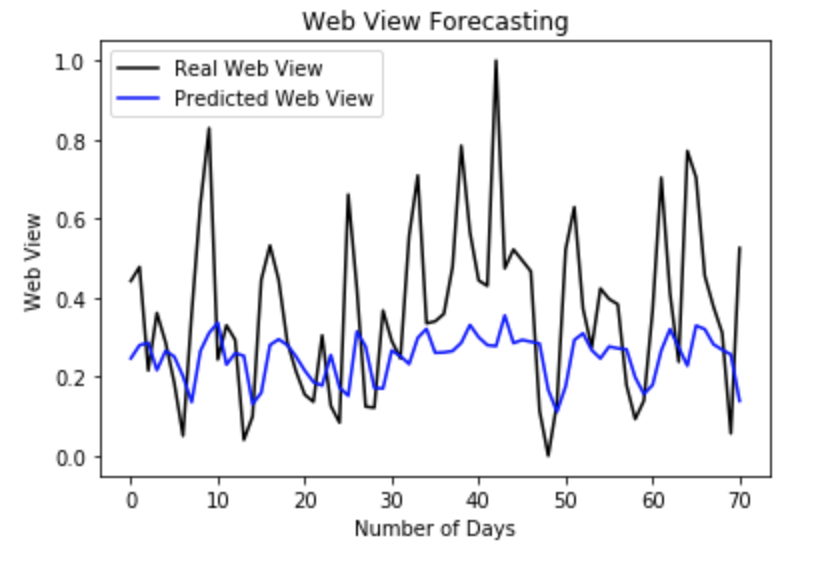
\includegraphics[height=6cm, width=10cm]{15}
\caption{15}
\end{figure}
       \end{frame}       
     \begin{frame}
    \frametitle{Model Fitting -- LSTM}
    \begin{figure}[htbp]
\centering
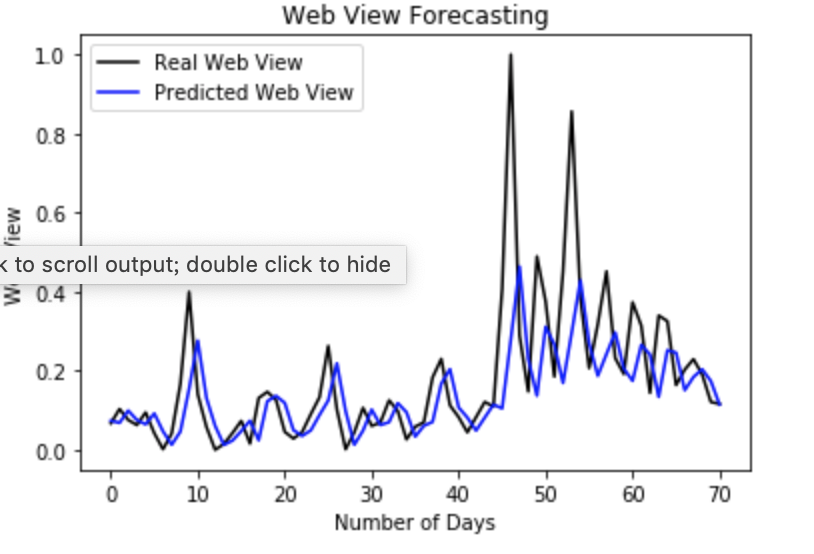
\includegraphics[height=6cm, width=10cm]{16}
\caption{16}
\end{figure}
       \end{frame}   
     \begin{frame}
    \frametitle{Model Fitting -- LSTM}
    \begin{figure}[htbp]
\centering
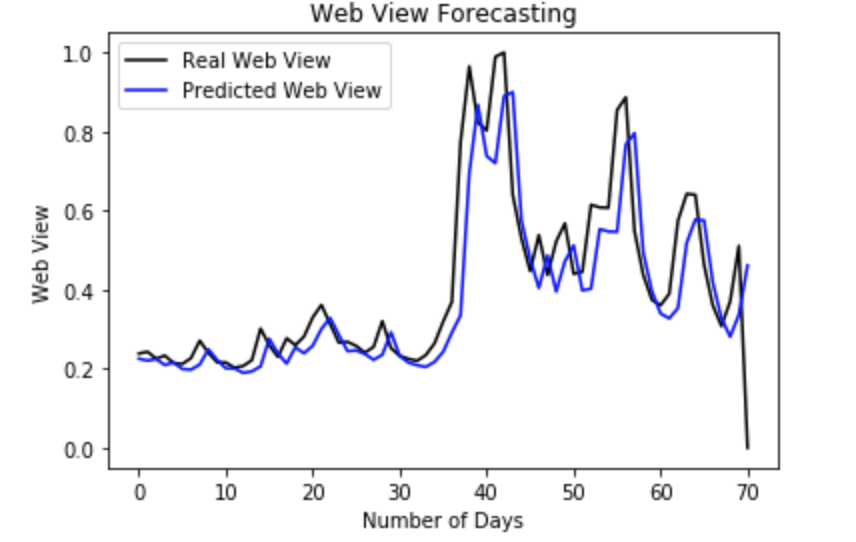
\includegraphics[height=6cm, width=10cm]{17}
\caption{17}
\end{figure}
       \end{frame}      
    
      \begin{frame} 
    \begin{center}
    \LARGE{{\color{red} {\bf Thank you!}}}
    \end{center}
    \end{frame}\end{CJK*}
\end{document}